\documentclass[a4paper]{article}
\usepackage{amsmath}
\usepackage{amsfonts}
\usepackage{amsthm}
\usepackage{amssymb}
\usepackage{mathtools}
\usepackage[english]{babel}
\usepackage{float}
\usepackage{graphicx}
\usepackage{hyperref}
\usepackage[utf8]{inputenc}
\usepackage{listings}
\usepackage{xcolor}
\usepackage{pdfpages}
\usepackage{graphicx}
\usepackage{subcaption}
\usepackage{stmaryrd}
\usepackage{a4wide}
\usepackage[nottoc]{tocbibind}
%% \usepackage{standalone}
\usepackage{subfiles}

\lstset{
  frame=tb,
  language=Python,
  aboveskip=3mm,
  belowskip=3mm,
  showstringspaces=false,
  formfeed=newpage,
  tabsize=4,
  comment=[l]{\#},
  breaklines=true,
  basicstyle=\small
}

\DeclarePairedDelimiter{\ceil}{\lceil}{\rceil}
\newcommand{\prob}[1]{\mathbb{P}\left(#1\right)}
\newcommand{\expect}[1]{\mathbb{E}\left(#1\right)}
\newcommand{\avg}[1]{\sum_{i=1}^{#1}X_i}
\newcommand{\dotpr}[2]{\langle #1,\; #2 \rangle}
\newcommand{\norm}[1]{\left\lVert#1\right\rVert}
\newcommand*{\QEDA}{\hfill\ensuremath{\blacksquare}}%

\def\biblio{\bibliographystyle{plain}\bibliography{mybib}}



\title{
  \vspace{-3cm} 
  \huge Project Outside the Course Scope \\
  \large Algorithms for Change Detection in Satellite Image Time Series
}
\author{Dmitry Serykh (qwl888)}

\begin{document}
\def\biblio{}

\maketitle
\tableofcontents
\newpage
%% \documentclass[main.tex]{subfiles}

\begin{document}
\chapter{Introduction}
\label{chap:intro}
\section{Motivation}
\label{sec:motivation}
Climate change is the defining issue of our time, and we are at a defining
moment \cite{un}. Without drastic and swift action in the nearest future, adapting to
these changes is becoming progressively more challenging. One way, in which we
can fight this development is by monitoring and reducing global deforestation.
If the areas of deforestation are registered in a timely fashion, targeted
countermeasures could be applied, and the tide on this trend could be turned. \\\\
Meanwhile, enormous amount of satellite data is becoming available to the earth
science community. This image data can, inter alia, be utilized for the
time-series based change-detection, which is a promising tool for monitoring and
mapping of deforestation and forest degradation. Most of these approaches
operate on individual pixels. Therefore, the sheer scale of this problem (being
hundreds of billions of pixels) becomes its most significant challenge, since
there are petabytes of image data being added on a yearly basis. Without
efficient data-parallel approaches, this approach quickly becomes infeasible in
practice, even when equipped with significant computational resources and
specialized hardware. \\\\
Recently, a novel massively-parallel implementation for a
change detection method has been proposed \cite{bfast_monitor}. It combines state-of-the-art methods
for the seasonal data change-detection with modern data-parallel programming
models and yields an implementation that makes the task feasible for giant sets.
Furthermore, this implementation is feasibly executable on consumer-grade
graphical processing hardware. The authors of the paper provide a
massively-parallel implementation for the BFAST-Monitor unsupervised change
detection algorithm. 
In this project, I will research alternative approaches to
BFAST-Monitor.

\section{BFAST}
\label{sec:changes}
Remotely sensed long term data is a valuable resource that was shown to be applicable for
change detection. There are three types of changes over time that are of
interest to the earth science research:
\begin{enumerate}
\item \textbf{Seasonal change}: changes that happen withing a season (e.g. year)
\item \textbf{Gradual change}: changes that are caused by interannual climate
  variability.
\item \textbf{Abrupt change}: rapid changes that are triggered by deforestation,
  floods, fires and similar.
\end{enumerate}
In the paper from 2010, Verbesselt et al. \cite{bfast}, describe an approach for
time series change detection, which involves
detection of multiple abrupt changes in the seasonal and trend components of the time series and
characterization of such changes by their magnitude and direction. The
piecewise linear model is assumed for the trend component and a
periodic models is applied to the seasonal component. The
coefficients for the linear models are estimated using ordinary least squares (OLS)
based linear regression.
This report covers the underlying theory and implementation of two algorithms based
on this approach (BFAST0n and BFAST).

\section{Contributions}
\label{sec:contributions}
The principal contributions of this project are: 

\begin{itemize}
\item I describe the underlying theory and concrete steps of the
  Seasonal and Trend decomposition using Loess (STL)
  time series decomposition algorithm, which is an essential part of BFAST.
  In particular, the description and values for all algorithm parameters are
  covered (Chapter \ref{chap:stl}).
\item Describe the underlying theory and link it to the concrete steps of
  the Ordinary Least Squares Moving Sum (OLS-MOSUM) test from the
  \texttt{strucchange} package \cite{strucchange} for the R programming
  language by Achim Zeileis. I also provide examples to illustrate the
  operation of the non-trivial parts of the algorithm. OLS-MOSUM test is another
  important building block of BFAST (Chapter \ref{chap:mosum}).
\item Describe the theory and algorithm steps of the multiple
  breakpoint estimation algorithm by Bai and Perron, based on the paper from 2003 \cite{bai_perron}
  and provide illustrative examples. This dynamic programming-based algorithm is
  an integral component of BFAST (Chapter \ref{chap:breakpoints}).
\item Describe the theory and steps of the BFAST and BFAST0n structural change
  detection algorithms by Jan Verbesselt et. al. \cite{bfast}. In particular,
  two seasonal models are explained in depth and matrix form of both models is
  provided (not included in the original paper).
  (Chapters \ref{chap:bfast} and \ref{chap:bfast0n}).
\item Provide and describe a prototype implementation of BFAST0n and BFAST in a
  general-purpose programming language (Python) (Chapter \ref{chap:implementation}).
\item Validate the implementation using simulated and real-life small
  datasets from the original paper by Verbesselt et al. \cite{bfast}.
  The results are compared to the original R implementation \cite{bfast-github}.
  (Chapter \ref{chap:validation}). 
\end{itemize}

\biblio
\end{document}


%% \documentclass[main.tex]{subfiles}

\begin{document}
\chapter{Seasonal Trend Decomposition (STL)}
\label{chap:stl}
STL, as first described by Cleveland et al. \cite{stl}, is an
algorithm for decomposition of time series, which is a common task in
statistics and used by the BFAST algorithm to get the initial estimate of the
seasonal componenet $\hat{S_t}$.
STL decomposes a time series $Y_v$ into three components:
\[
Y_v = T_v + S_v + R_v \text{ for } v \in 1..N
\]
where:
\begin{itemize}
\item $T_v$ is the trend component, which captures the long-term progression of
  the time-series
\item $S_v$ is the seasonal component, which reflects the seasonal variation of
  the data
\item $R_v$ is the remainder(residual) component, which is the remaining variation of the time series
\end{itemize}
An example of such decomposition is illustrated on Figure \ref{fig_stl}.
STL alone, however, can not be used for break detection because it uses smoothing
that would temper with the breakpoint information. Therefore, it is only used in
the pre-processing stage to get the initial estimate of the seasonal component.
\begin{figure}
  \centering
  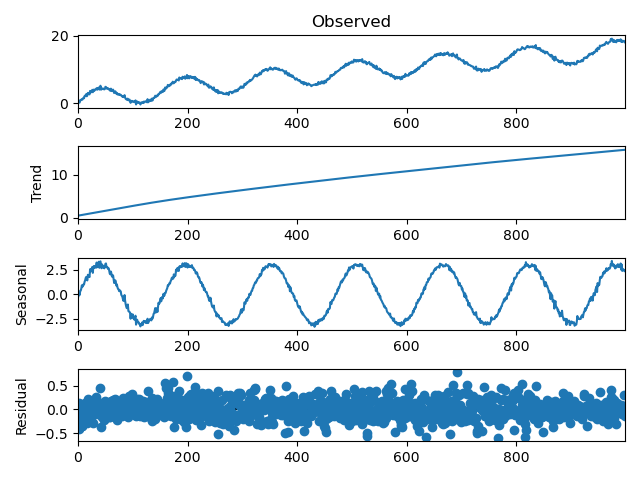
\includegraphics[width=0.7\textwidth]{imgs/stl1}
  \caption{STL applied to $f(x) = x^{0.75} + 2\sin(x)$ with added Gaussian noise
    $\sim \mathcal{N}(0, 0.25)$ and $n = 1000$. It can be seen that
    $T_v \approx v^{0.75}$, $S_v \approx 2\sin(v)$ and $R_v \sim \mathcal{N}(0, 0.25)$. }
  \label{fig_stl}
\end{figure}


\section{Locally Weighted Regression (LOESS)}
\label{sec:locally_weighted_running_line_smoother}
The key component of the STL method is the Locally Weighted Regression (LOESS),
that is described in \cite{loess} and \cite{stl}. LOESS is a robust smoothing method that is
commonly used in statistics and operates as follows:
\begin{itemize}
\item We have a set of $(x_i, y_i)$ for $1 \leq i \leq n$.
\item We wish for all $x$ fit a curve $\hat{g}(x)$ by giving the other points $x_i$ a
  weight $v_i$.
\item We select a value of $q \in \mathbb{Z}^+$
\item Let $\lambda_q(x)$ be the distance from $x$ to q'th closest $x_i$.
  This definition would not, however, work when $q > n$. In that case, we must
  apply scaling by setting:
  \[
  \lambda_q(x) = \frac{q \cdot \lambda_n(x)}{n}
  \]
\item We calculate the weights using the tricube weight function:
  \[
  v_i = \left( 1 - \left( \frac{| x_i - x |}{\lambda_q(x)}  \right)^3\right)^3
  \]
  we also add a low shelf, for $| x_i - x | \geq \lambda_q(x)$, we set $v_i = 0$
\item We then use locally-linear or locally quadratic fitting with weights
  $\rho_i v_i$, where $\rho_i$ are the robustness weights, used by the STL.
  Addition of $\rho_v$ is crucial, since it allows us to ignore the outliers
  in the dataset. This way, we introduce robustness into STL.
  The value of locally-fitted polynomial at $x$ is $\hat{g}(x)$, and $d$ is
  the degree of the fitted polynomial.
\end{itemize}
In this algorithm, $q$ is the smoothing factor. The higher the value of $q$ is, the more
the curve resembles a fitted polynomial of degree $d$ for all $x$. Another
important parameter is the value of $d$. Cleveland et al.
\cite{stl} suggest using $d \in \{1,2\}$ for STL. Value of $2$ is used when the
function of interest has a more pronounced curvature. An example of the usage of
LOESS smoothing can be seen on Figure \ref{fig_loess}.

\begin{figure}
  \centering
  \begin{subfigure}[b]{0.49\textwidth}
    \centering
    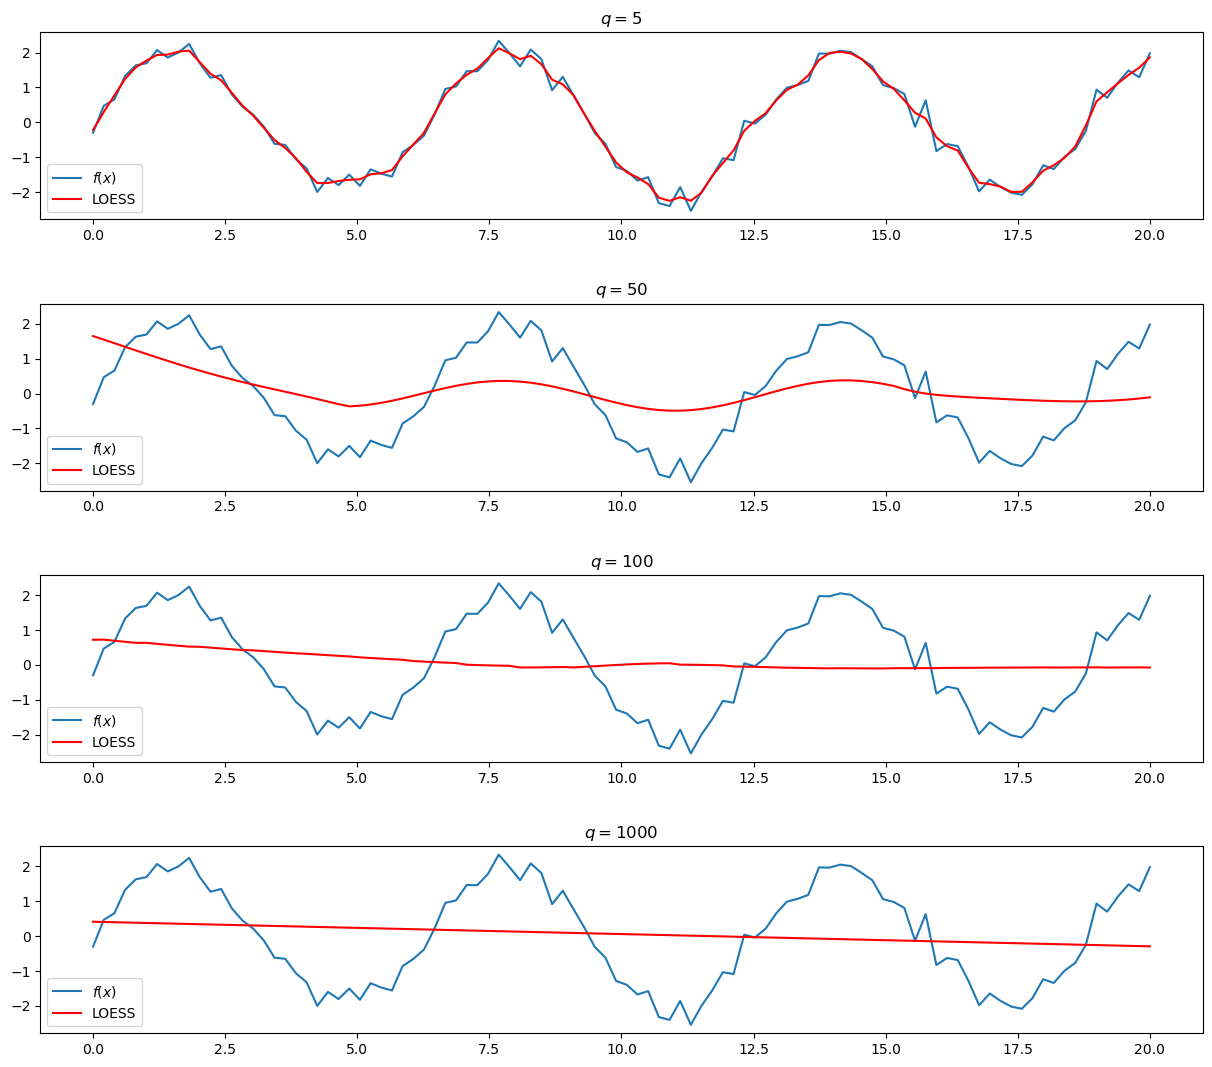
\includegraphics[width=\textwidth]{imgs/loess1}
    \caption{$d=1$}
  \end{subfigure}
  \begin{subfigure}[b]{0.49\textwidth}
    \centering
    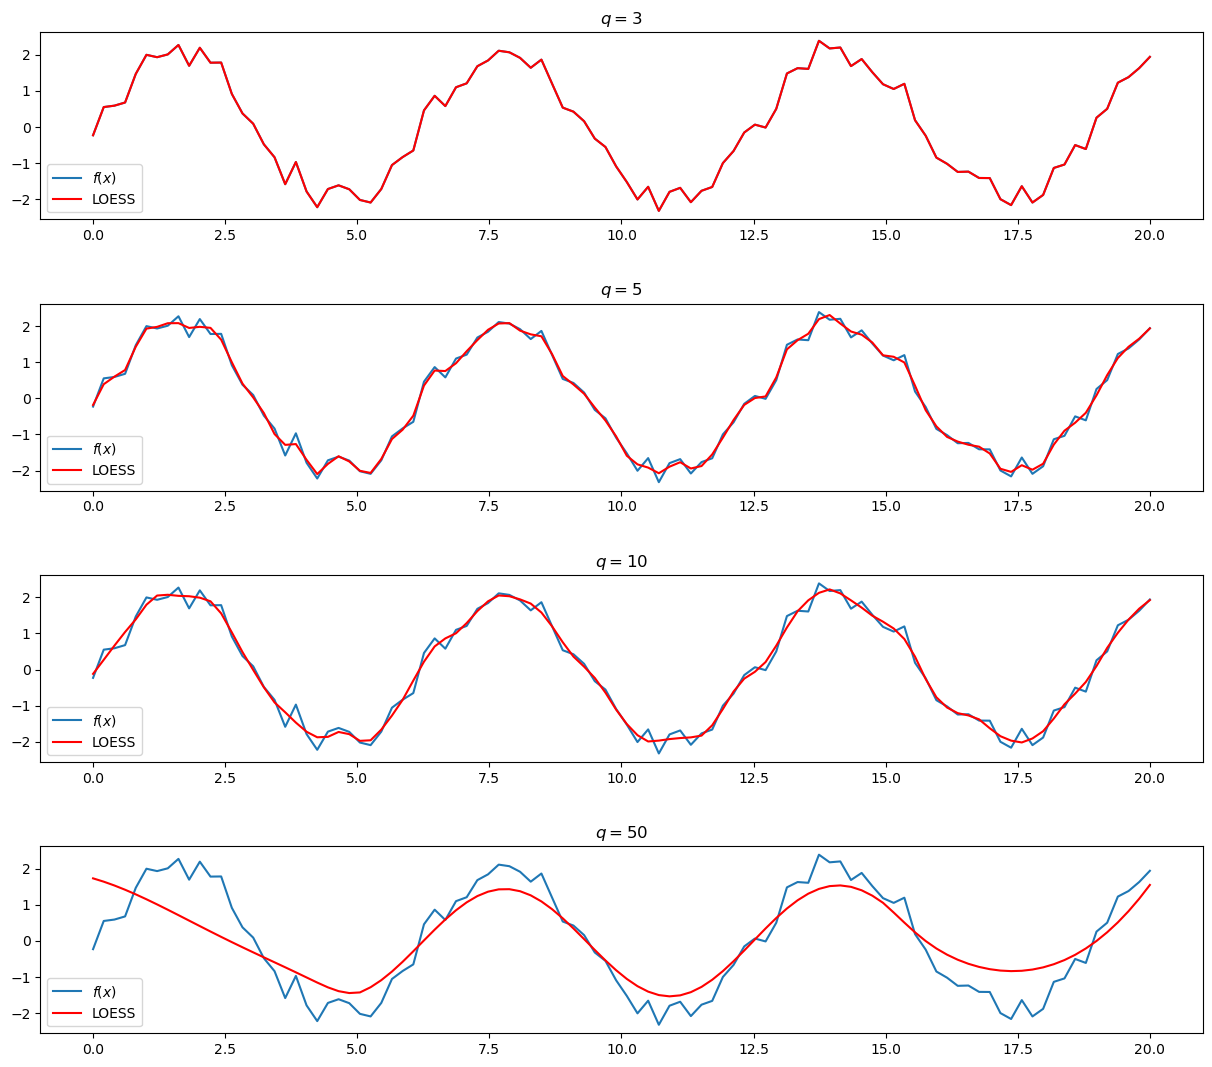
\includegraphics[width=\textwidth]{imgs/loess2}
    \caption{$d=2$}
  \end{subfigure}
  \caption{LOESS applied to $f(x) = 2\sin(x)$ with added Gaussian noise and $n = 100$}
  \label{fig_loess}
\end{figure}

\section{The Incremental Algorithm}
\label{sec:the_incremental_algorithm}
STL is performed through two nested loops and we begin by setting:
\begin{align*}
  T_v^{0} &= 0\\
  R_v^{0} &= 0\\
  \rho_v &= 1
\end{align*}
\subsection{Inner loop}
\label{subsec:inner_loop}
The inner loop consists of following steps:
\begin{enumerate}
\item \textbf{Detrending}:
  $Y_v - T_v^k$, where $k$ is the iteration number. Note however,
  that if a value of $Y_v$ is missing, the detrending value must also be missing.
\item \textbf{Cycle-Subseries Smoothing}:
  $Y_v - T_v^k$ is split into cycle-subseries. LOESS with $q=n_s$ and $d=1$ is
  applied to each cycle-subseries, resulting in $C^{k+1}$.
\item \textbf{Low-pass Filter of Smoothed Cycle-Subseries}:
  Apply the low-pass filter to $C_{k+1}$. This is accomplished by application of two
  moving averages of lag equal to 3 followed by LOESS smoothing with $q=n_l$
  and $d=1$.
  The result is saved as $L^{k+1}$
\item \textbf{Detrending of the Smoothed Cycle-Subseries}:
  $S^{k+1} = C^{k+1} - L^{k+1}$
\item \textbf{Deseasoning}:
  $Y_v - S_v^k$. If a value of $Y_v$ is missing, the detrending value must also be missing.
\item \textbf{Trend Smoothing}:
  Apply LOESS to $Y_v - S_v^k$ with $q = n_t$, resulting in $T^{k+1}$
\end{enumerate}

\subsection{Outer loop}
\label{subsec:outer_loop}
The outer loop consists of following steps:
\begin{enumerate}
\item Run the inner loop
\item Find the remainder:
  $R_v = Y_v - T_v - S_v$
\item Calculate the robustness weights from the remainder component:
  \[
  \rho_{v}= B\left( \frac{|R_v|}{6\cdot\text{median}(|R_v|)} \right)
  \]
  where $B$ is the bisquare weight function:
  \[
  B(x) =
  \begin{cases}
    \left(1-x^{2}\right)^{2} & \text{ for } 0 \leqslant x<1 \\
     0                     & \text{ for } x>1
  \end{cases}
\]
\end{enumerate}

\section{Parameters and Their Values}
\label{sec:parameter_values}
STL has following parameters \cite{stl}:
\begin{enumerate}
\item $n_p$ : period of the seasonal component in number of observations.
  Specific for each data set.
\item $n_i$ : number of inner loop iterations. \texttt{stlplus}, which is
  popular STL library that is used in the BFAST R implementation \cite{bfast-github}, uses a
  value of $n_i = 2$ \cite{stlplus}.
\item $d$: degree for the polynomials that is being fitted.
  \texttt{stlplus} uses a value of $d=1$ for all smoothing.
\item $n_o$ : number of the outer loop iterations. The default value in
  \texttt{stlplus} is 1. This can be adjusted if outliers are present in the dataset.
\item $n_l$ : value of the smoothing parameter ($q$) for the LOESS procedure in the
  \textbf{Low-pass filter} stage of the inner loop. Typically (which includes
  \texttt{stlplus}), $n_l$ is the smallest odd integer greater than the period.
\item $n_t$ : value of $q$ for the trend component, which should be odd.
  \texttt{stlplus} uses following:
  \[
  n_t =\text{nextodd}\left(
  \ceil[\bigg]{
    \frac{1.5 \cdot n_p}
         {1-1.5/n_s}
  }
  \right)
  \]
\item $n_s$ : value of $q$ for the seasonal component. According to Cleveland
  et al. \cite{stl}, it must be specifically and
  carefully chosen for each application. \texttt{stlplus} allows
  the user to select $n_s = \text{``\emph{periodic}''}$, which is, according to
  the package documentation \cite{stlplus}, almost equivalent to replacing
  the smoothing in the seasonal component with taking the mean. It is the value,
  used by the BFAST R-implementation and consequently for this project.
\end{enumerate}
\biblio
\end{document}


%% \documentclass[presentation.tex]{subfiles}

\begin{document}

\begin{frame}
\frametitle{OLS-MOSUM Test - The Model}
\begin{itemize}
  \item One step of the BFAST algorithm is to detect structural change in the
    trend and seasonal components before we commit to the heavy-weight
    estimation of the number and location of the breakpoints.
  \item For each observation $i \in (1, \ldots, n)$ we consider a following linear model:
    \[
    y_{i}=x_{i}^{\top} \beta_{i}+u_{i}
    \]
    where:
    \begin{itemize}
    \item $x_i = (1,x_{i2}, x_{i3}, ..., x_{ik})^T \in \mathbb{R}^k$
    \item $u_i \in \mathbb{R}$ is the residual term that is independently and identically
      distributed with mean $\mu = 0$ and variance $\sigma^2$.
    \end{itemize}
  \item 
    We can then test for structural change by testing the null hypothesis:
    \[
    H_0:\quad \beta_i = \beta_0 \quad(i=1, \ldots, n)
    \]
\end{itemize}
\end{frame}

\begin{frame}
  \frametitle{OLS-MOSUM Test - Continued}
  \begin{itemize}
  \item $\hat{\beta}^{(n)}$ is the ordinary least squares (OLS) estimate of the
    regression coefficients based on all the observations up to $n$,
  \item 
    Let the OLS residuals (estimates of $u_i$) be defined as:
    \begin{equation} \label{eq:residuals}
      \hat{u}_i = y_i - x_i^T\hat{\beta}^{(n)}
    \end{equation}
    the variance estimate would then be:
    \begin{equation} \label{eq:sigma}
      \hat{\sigma}^{2}=\frac{1}{n-k} \sum_{i=1}^{n} \hat{u}_{i}^{2}
    \end{equation}
  \end{itemize} 
\end{frame}

\begin{frame}
  \frametitle{Empirical Fluctuation Process (OLS-MOSUM)}
  \begin{itemize}
  \item It is possible to detect structural change by analyzing moving sum of residuals ($\hat{u}$)
  \item 
    The resulting empirical fluctuation process consists of a
    sum of a fixed number of residuals in a data interval, which size is determined
    by the value of the parameter $h \in (0,1)$ (bandwidth).
  \item 
  The OLS-based MOSUM process at time $t$ is given by:
  \begin{equation}\label{eq:mosum_og}
    M(t)=\frac{1}{\hat{\sigma} \sqrt{n}}
    \left(\sum_{i=\floor{N_{n} t}+1}^{\left\lfloor N_{n} t\right\rfloor+\lfloor
      n h\rfloor} \hat{u}_{i}\right) \quad(0 \leq t \leq 1-h)
  \end{equation}
  where $N_{n}=(n-\floor{n h}) /(1-h)$ and $\floor{n h}$ is the size of the
  window. 
  \end{itemize}
\end{frame}

\begin{frame}
  \frametitle{Significance Testing}
  \begin{itemize}
  \item 
    A key observation is that if a structural change takes place at $t_0$, the
    OLS-MOSUM path would also have a strong shift at $t_0$.
    We reject the null hypothesis of there being no structural change, when the fluctuation of
    the OLS-MOSUM process becomes too large.
  \item
    In practice, we determine whether the null
    hypothesis can be rejected using a significance test (also called statistical
    hypothesis testing).
  \item 
    First, we calculate the test statistic. For the residual-based OLS-MOSUM
    process, it is defined as:
    \begin{equation} \label{eq:test_statistic_og}
      S_{\text{MOSUM}} = \max(|M(t)|) \quad \text{ for } 0 \leq t \leq (1-h)
    \end{equation}
  \end{itemize}
\end{frame}

\begin{frame}
  \frametitle{Significance Testing - Continued}
  \begin{itemize}
  \item This formulation is not usable in a context of an implementation, since we are working
    with infinite set of real numbers from $0$ to $1-h$.
  \item Another key observation is that $M(t)$ returns $n - \floor{nh} + 1$ unique values for $0 \leq t \leq (1-h)$:
  \item Let:
    \begin{equation} \label{eq:mosum}
      \bar{M}(t') =
      \frac{1}{\hat{\sigma} \sqrt{n}}
      \left(\sum_{i=t}^{t' + \floor{nh}} \hat{u}_i\right)
      \quad(t' = 1,2, \hdots, n - \floor{nh} + 1))
    \end{equation}
  \item Then: 
    $\max(|M(t)|) = \max(|\bar{M}(t')|)$ and we have:
    \begin{equation} \label{eq:test_statistic}
      S_{\text{MOSUM}} = \max(|\bar{M}(t')|) \quad \text{ for } t' \text{ in } 1,2,..,(n - \floor{nh} + 1)
    \end{equation}
  \end{itemize}
\end{frame}

\begin{frame}
  \frametitle{Significance Testing - Continued 2}
  \begin{itemize}
  \item We use the value of $S_{\text{MOSUM}}$ to calculate the probability of getting such
    sample, given that the null hypothesis holds, using the critical values approach.
    The p-value is calculated from the table of
    simulated asymptotic critical values of the Moving Estimate (ME) tests with
    the maximum norm, given by Chu et al. (1995).
  \item  We then compare the resulting
    probability with a chosen confidence interval, which is a value $0 < \alpha < 1$
    \item If the resulting probability is below the
      value of $\alpha$, we reject the null hypothesis, hence a 
      structural change is detected in the time series. 
  \end{itemize}
\end{frame}

%% \begin{frame}[fragile]
%%   \frametitle{Table of Critical Values}
%%   \begin{table}[]
%%     \centering
%% \begin{tabular}{|l|l|l|l|l|l|}
%% \hline
%% \multirow{2}{*}{$k$}      & \multicolumn{1}{c|}{\multirow{2}{*}{h}} & \multicolumn{4}{c|}{Tail probability}                                                                     \\ \cline{3-6} 
%%                           & \multicolumn{1}{c|}{}                   & 0.10                     & 0.05                     & 0.025                    & 0.01                     \\ \hline
%% \multirow{4}{*}{1}        & 0.05                                    & 0.7552                   & 0.8017                   & 0.8444                   & 0.8977                   \\ \cline{2-6} 
%%                           & 0.10                                    & 0.9809                   & 1.0483                   & 1.1119                   & 1.1888                   \\ \cline{2-6} 
%%                           & \multicolumn{1}{c|}{...}                & \multicolumn{1}{c|}{...} & \multicolumn{1}{c|}{...} & \multicolumn{1}{c|}{...} & \multicolumn{1}{c|}{...} \\ \cline{2-6} 
%%                           & 0.50                                    & 1.3560                   & 1.4938                   & 1.6166                   & 1.7663                   \\ \hline
%% \multirow{4}{*}{2}        & 0.05                                    & 0.7997                   & 0.8431                   & 0.8838                   & 0.9351                   \\ \cline{2-6} 
%%                           & 0.10                                    & 1.0448                   & 1.1067                   & 1.1634                   & 1.2388                   \\ \cline{2-6} 
%%                           & \multicolumn{1}{c|}{...}                & \multicolumn{1}{c|}{...} & \multicolumn{1}{c|}{...} & \multicolumn{1}{c|}{...} & \multicolumn{1}{c|}{...} \\ \cline{2-6} 
%%                           & 0.50                                    & 1.4884                   & 1.6125                   & 1.7266                   & 1.8639                   \\ \hline
%% \multicolumn{1}{|c|}{...} & \multicolumn{1}{c|}{...}                & \multicolumn{1}{c|}{...} & \multicolumn{1}{c|}{...} & \multicolumn{1}{c|}{...} & \multicolumn{1}{c|}{...} \\ \hline
%% \end{tabular}
%% \caption{An excerpt from the table of simulated asymptotic critical values of the
%%   ME tests with the maximum norm}
%% \label{table:critvals}
%% \end{table}
%% \end{frame}


\begin{frame}[fragile]
  \frametitle{OLS-MOSUM Test - Steps of the Algorithm}
  \begin{enumerate}
  \item \textbf{Calculate $\hat{\beta}^{(n)}$ using OLS-based linear
    regression from matrix $\mathrm{X}$ and vector $y$}
  \item \textbf{Calculate the vector of OLS residuals $\hat{\mu}$}
  \item \textbf{Calculate the standard deviation $\hat{\sigma}$}
  \item \textbf{Calculate the residual-based OLS-MOSUM process as a vector of size $n - \floor{nh} + 1$}
  \begin{verbatim}
  nh = floor(n * h)
  e = concat([0], residuals)
  process = cumsum(e)
  process = process[nh:n] - process[0:(n - nh + 1)]
  process = process / (sigma * sqrt(n))
  \end{verbatim}
\item \textbf{Calculate the test statistic $S_{\text{test}}$} = \texttt{max(abs(process))}
\item \textbf{Calculate the p-value using the table of critical values and linear interpolation}
\item \textbf{Return the result}: \\
  If $p \leq \alpha$, we reject the null-hypothesis. Structural change is detected
  \end{enumerate} 
\end{frame}




\end{document}

\subfile{mosum.tex}

%% \documentclass[presentation.tex]{subfiles}

\begin{document}

\begin{frame}
\frametitle{Breakpoint Estimation - Intro}
\begin{itemize}
  \item Described in the paper by Bai and Perron from 2003
  \item Estimate the number and position of breakpoints in a time series using
    a dynamic programming algorithm and Bayesian Information Criterion (BIC)
\end{itemize}
\end{frame}


\begin{frame}
\frametitle{Breakpoint Estimation - The Model}
\begin{itemize}
  \item 
We assume a pure structural change model for $m$ breaks ($m+1$ segments):
\[
y_{t} = x_{t}^{\top} \beta_{j}+u_{t} \quad t=T_{j-1}+1, \ldots, T_{j}
\]
for $j = 1,\hdots , m+1$, and where:
\vspace{2.5mm}
\begin{itemize}
\item $x_t \in \mathbb{R}^q$ is the value of the independent variable at time
  $t = 1,\hdots , T$
\item $y_{t} \in \mathbb{R}$ is the observation at time $t$
\item $\beta_j: \; (j=1, \hdots ,m+1)$ is the vector of coefficients for the segment $j$
\item $u_{t} \in \mathbb{R}$ is the disturbance (error) at time $t$
\item $(T_1, \hdots ,T_m)$ are the unknown indices of the $m$ breakpoints.
 We additionally set $T_0 = 0$ and $T_{m+1} = T$
\end{itemize}
\item 
In other words, we split the time series into $m+1$ segments (of potentially
different sizes) and perform linear
regression independently for each segment, where for segment $i$, we estimate
a coefficient vector $\beta_i$.
Hence, we find the estimate of the coefficient vector ($\hat{\beta}$) for each
m-partition $(T_1, ..., T_m)$ by minimizing the sum of squared residuals:
\[
\sum_{i=1}^{m+1}\sum_{i=T_{i-1} + 1}^{T_i} \left[ y_t - x_t^{\top}\beta_i \right]^2
\]
\end{itemize}
\end{frame}

\begin{frame}
  \frametitle{}
\begin{itemize}
\item
Let $\{T_j\}$ denote an m-partition $(T_1, ..., T_m)$ and $S_T(T_1, ..., T_m)$
denote the resulting sum of squared residuals. Since we can estimate the
coefficient vector for each partition, we can minimize the sum of
squared residuals by finding the optimal position for the breakpoints
\[
(\hat{T}_1, ..., \hat{T}_m) = \operatorname{argmin}_{T_{1}, \ldots, T_{m}}
S_{T}\left(T_{1}, \ldots, T_{m}\right)
\]
\item
There is a finite number of possible breakpoints, and only a subset of
possible partitions is feasible. There are $T(T+1)/2$ (sum of integers from 1 to T)
possible segments that can be chosen. This can be demonstrated by building a
matrix of possible segments, with starting date on the y-axis and terminal date
on the y-axis. A length of a segment is positive, hence we can eliminate
one half of the potential segments. There are further reductions
that can be made that reduce the number of feasible segments to
$T(T+1)/2 - \left(T(h-1)-m h(h-1)-(h-1)^{2}-h(h-1) / 2\right)$, where $h$ is the minimal
segment length.
\end{itemize}
\end{frame}

\begin{frame}[fragile]
  \frametitle{Upper-diagonal Matrix of Sums of Squared Residuals}
\begin{table}[]
\begin{tabular}{lllllllllll}
                                   & \multicolumn{10}{c}{stop}                                                                                                                                                                                                                                                 \\ \cline{2-11} 
\multicolumn{1}{l|}{}              & \multicolumn{1}{l|}{}  & \multicolumn{1}{l|}{1}    & \multicolumn{1}{l|}{2}    & \multicolumn{1}{l|}{3}    & \multicolumn{1}{l|}{4}    & \multicolumn{1}{l|}{5}    & \multicolumn{1}{l|}{6}    & \multicolumn{1}{l|}{7}    & \multicolumn{1}{l|}{8}    & \multicolumn{1}{l|}{9}    \\ \cline{2-11} 
\multicolumn{1}{l|}{}              & \multicolumn{1}{l|}{1} & \multicolumn{1}{l|}{$\operatorname{nf}_1$} & \multicolumn{1}{l|}{$\operatorname{nf}_1$} & \multicolumn{1}{l|}{$\operatorname{nf}_1$} & \multicolumn{1}{l|}{f}   & \multicolumn{1}{l|}{f}   & \multicolumn{1}{l|}{f}   & \multicolumn{1}{l|}{$\operatorname{nf}_2$} & \multicolumn{1}{l|}{$\operatorname{nf}_2$} & \multicolumn{1}{l|}{$\operatorname{nf}_2$} \\ \cline{2-11} 
\multicolumn{1}{l|}{}              & \multicolumn{1}{l|}{2} & \multicolumn{1}{l|}{}     & \multicolumn{1}{l|}{$\operatorname{nf}_1$} & \multicolumn{1}{l|}{$\operatorname{nf}_1$} & \multicolumn{1}{l|}{$\operatorname{nf}_1$} & \multicolumn{1}{l|}{$\operatorname{nf}_3$} & \multicolumn{1}{l|}{$\operatorname{nf}_3$} & \multicolumn{1}{l|}{$\operatorname{nf}_2$} & \multicolumn{1}{l|}{$\operatorname{nf}_2$} & \multicolumn{1}{l|}{$\operatorname{nf}_2$} \\ \cline{2-11} 
\multicolumn{1}{l|}{}              & \multicolumn{1}{l|}{3} & \multicolumn{1}{l|}{}     & \multicolumn{1}{l|}{}     & \multicolumn{1}{l|}{$\operatorname{nf}_1$} & \multicolumn{1}{l|}{$\operatorname{nf}_1$} & \multicolumn{1}{l|}{$\operatorname{nf}_1$} & \multicolumn{1}{l|}{$\operatorname{nf}_3$} & \multicolumn{1}{l|}{$\operatorname{nf}_2$} & \multicolumn{1}{l|}{$\operatorname{nf}_2$} & \multicolumn{1}{l|}{$\operatorname{nf}_2$} \\ \cline{2-11} 
\multicolumn{1}{l|}{start} & \multicolumn{1}{l|}{4} & \multicolumn{1}{l|}{}     & \multicolumn{1}{l|}{}     & \multicolumn{1}{l|}{}     & \multicolumn{1}{l|}{$\operatorname{nf}_1$} & \multicolumn{1}{l|}{$\operatorname{nf}_1$} & \multicolumn{1}{l|}{$\operatorname{nf}_1$} & \multicolumn{1}{l|}{f}   & \multicolumn{1}{l|}{f}   & \multicolumn{1}{l|}{f}   \\ \cline{2-11} 
\multicolumn{1}{l|}{}              & \multicolumn{1}{l|}{5} & \multicolumn{1}{l|}{}     & \multicolumn{1}{l|}{}     & \multicolumn{1}{l|}{}     & \multicolumn{1}{l|}{}     & \multicolumn{1}{l|}{$\operatorname{nf}_1$} & \multicolumn{1}{l|}{$\operatorname{nf}_1$} & \multicolumn{1}{l|}{$\operatorname{nf}_1$} & \multicolumn{1}{l|}{f}   & \multicolumn{1}{l|}{f}   \\ \cline{2-11} 
\multicolumn{1}{l|}{}              & \multicolumn{1}{l|}{6} & \multicolumn{1}{l|}{}     & \multicolumn{1}{l|}{}     & \multicolumn{1}{l|}{}     & \multicolumn{1}{l|}{}     & \multicolumn{1}{l|}{}     & \multicolumn{1}{l|}{$\operatorname{nf}_1$} & \multicolumn{1}{l|}{$\operatorname{nf}_1$} & \multicolumn{1}{l|}{$\operatorname{nf}_1$} & \multicolumn{1}{l|}{f}   \\ \cline{2-11} 
\multicolumn{1}{l|}{}              & \multicolumn{1}{l|}{7} & \multicolumn{1}{l|}{}     & \multicolumn{1}{l|}{}     & \multicolumn{1}{l|}{}     & \multicolumn{1}{l|}{}     & \multicolumn{1}{l|}{}     & \multicolumn{1}{l|}{}     & \multicolumn{1}{l|}{$\operatorname{nf}_1$} & \multicolumn{1}{l|}{$\operatorname{nf}_1$} & \multicolumn{1}{l|}{$\operatorname{nf}_1$} \\ \cline{2-11} 
\multicolumn{1}{l|}{}              & \multicolumn{1}{l|}{8} & \multicolumn{1}{l|}{}     & \multicolumn{1}{l|}{}     & \multicolumn{1}{l|}{}     & \multicolumn{1}{l|}{}     & \multicolumn{1}{l|}{}     & \multicolumn{1}{l|}{}     & \multicolumn{1}{l|}{}     & \multicolumn{1}{l|}{$\operatorname{nf}_1$} & \multicolumn{1}{l|}{$\operatorname{nf}_1$} \\ \cline{2-11} 
\multicolumn{1}{l|}{}              & \multicolumn{1}{l|}{9} & \multicolumn{1}{l|}{}     & \multicolumn{1}{l|}{}     & \multicolumn{1}{l|}{}     & \multicolumn{1}{l|}{}     & \multicolumn{1}{l|}{}     & \multicolumn{1}{l|}{}     & \multicolumn{1}{l|}{}     & \multicolumn{1}{l|}{}     & \multicolumn{1}{l|}{$\operatorname{nf}_1$} \\ \cline{2-11} 
\end{tabular}
\caption{An example of an upper-triangular matrix of sums of squared residuals for $T =
  9$, $h=3$, $m=2$. We must compute sum of squared residuals for all feasible
  segments (f).
}
\end{table}
\end{frame}



%% \begin{frame}
%%   \frametitle{Breakpoint Estimation - The Model Continued}
%%   \begin{itemize}
%%     \item 
%% This linear regression system can also be expressed in matrix form:
%% \[
%% Y = \overline{X}\beta + U
%% \]
%% where:
%% \[
%% Y =
%% \begin{bmatrix}
%% y_1 \\
%% y_2 \\
%% \vdots \\
%% y_T
%% \end{bmatrix}
%% \quad
%% \beta =
%% \begin{bmatrix}
%% \vert & \vert &  & \vert \\
%% \beta_{1} & \beta_{2}  & \hdots & \beta_{m+1}\\
%% \vert & \vert &  & \vert\\
%% \end{bmatrix}
%% \quad
%% U =
%% \begin{bmatrix}
%% u_1 \\
%% u_2 \\
%% \vdots \\
%% u_T
%% \end{bmatrix}
%% \]
%% and $\overline{X}$ is a block matrix that
%% diagonally partitions $X$ at breaking points $(T_1,..., T_m)$:
%% \[
%% \overline{X} =
%% \begin{bmatrix}
%% X_1 & 0 & \hdots & 0\\
%%  0 & X_2 & \hdots & 0 \\
%% \vdots & \vdots & \ddots & \vdots \\
%%  0 & 0 & \hdots & X_{m+1} 
%% \end{bmatrix}
%% \quad
%% X_i = 
%% \begin{bmatrix}
%%   \text{---} \hspace{-0.2cm} & x_{T_{i-1} + 1}^{\top} & \hspace{-0.2cm}\text{---} \\
%%   \text{---} \hspace{-0.2cm} & x_{T_{i-1} + 2}^{\top} & \hspace{-0.2cm}\text{---} \\
%%   & \vdots & \\ 
%%  \text{---} \hspace{-0.2cm} & x_{T_i}^{\top} & \hspace{-0.2cm}\text{---}  \\
%% \end{bmatrix}
%% \]
%% \end{itemize}  
%% \end{frame}

\end{document}


%% \documentclass[main.tex]{subfiles}

\begin{document}
\chapter{BFAST0N}
\label{chap:bfast0n}
The BFAST0N algorithm is the light-weight version of the BFAST approach that is based on
the application of the \texttt{breakpoints} function from the
\texttt{strucchange} package, which is described in Chapter
\ref{chap:breakpoints}.
\section{Harmonic model}
\label{sec:harmonic_model}

\section{Steps of the Algorithm}
\label{sec:bfast0n_algorithm_steps}

\section{Parameters and Their Values}
\label{sec:bfast0n_params}

\biblio
\end{document}


%% \documentclass[presentation.tex]{subfiles}

\begin{document}


\begin{frame}
  \frametitle{Structural Changes in Time Series Models}
  There are three types of changes over time that are of
    interest to the earth science research:
    \begin{enumerate}
    \item \textbf{Seasonal change}: changes that happen within a season (e.g. year)
    \item \textbf{Gradual change}: changes that are caused by interannual climate
      variability.
    \item \textbf{Abrupt change}: rapid changes that are triggered by deforestation,
      floods, fires and similar.
    \end{enumerate}
\end{frame}

\begin{frame}
  \frametitle{BFAST}
  \begin{itemize}
    \item 
      In the paper from 2010, Verbesselt et. al outline a generic change detection approach
      that combines iterative decomposition into trend, seasonal and remainder components and detection
      and characterizing of breakpoints within the trend and seasonal components.
    \item 
      For BFAST, we consider a following data model:
      \[
      Y_t = T_t + S_t + R_t, \quad t = 1,...,n
      \]
      where:
      \begin{itemize}
      \item $Y_t$ is the observation at time $t$
      \item $T_t$ is the trend component at time $t$
      \item $S_t$ is the seasonal component at time $t$
      \item $R_t$ is the remainder component at time $t$
      \item $n$ is the number of observations in time series
      \end{itemize}
  \end{itemize}
\end{frame}

\begin{frame}
\frametitle{BFAST Example - \texttt{harvest}}
\begin{figure}[H]
  \centering
  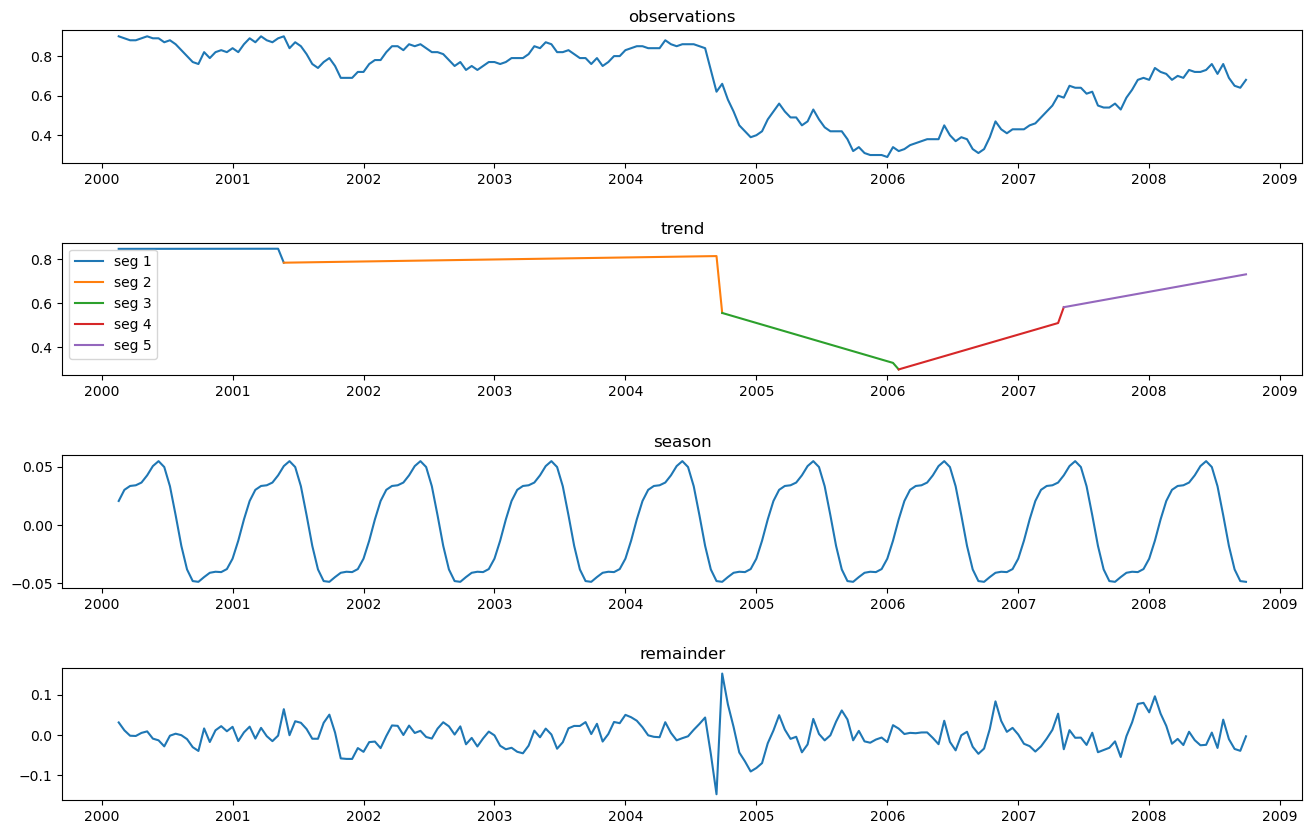
\includegraphics[width=0.9\textwidth]{imgs/harvest.png}
  \caption{Normalized Difference Vegetation Index (NDVI) time series for a pine plantation,
    with 23 observation per year. NDVI is an estimate of the density of green on an area of land.
    There are 4 breakpoints in the trend component. Harmonic seasonal model}
\end{figure}
\end{frame}


\begin{frame}
\frametitle{BFAST Example - \texttt{simts}}
\begin{figure}[H]
  \centering
  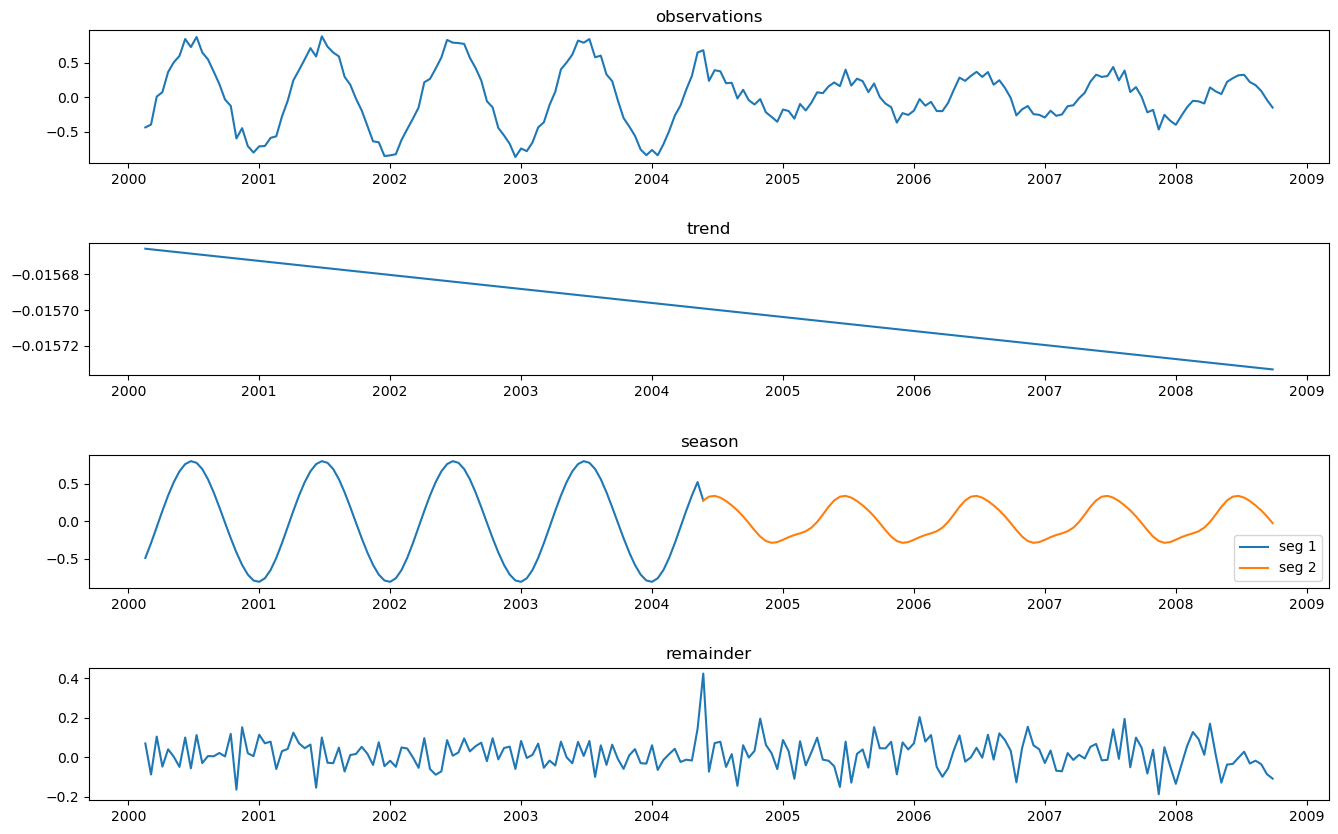
\includegraphics[width=0.9\textwidth]{imgs/simts.png}
  \caption{Simulated seasonal 16-day NDVI time series. The seasonal
    component has a single breakpoint. Harmonic seasonal model}
\end{figure}
\end{frame}

\begin{frame}
\frametitle{BFAST Example - \texttt{nile}}
\begin{figure}[H]
  \centering
  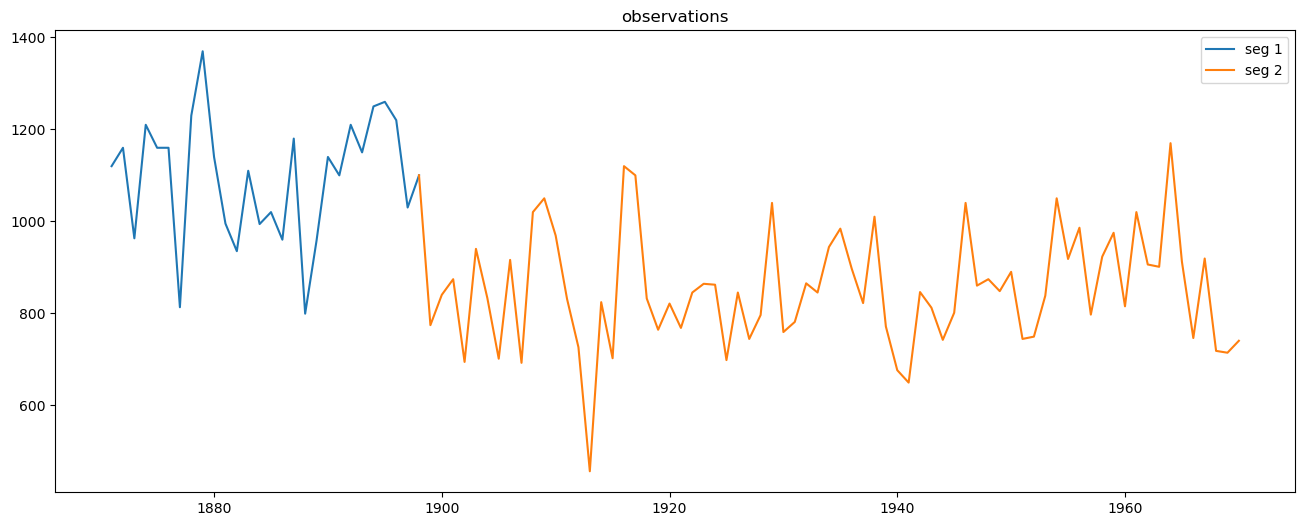
\includegraphics[width=0.9\textwidth]{imgs/nile.png}
  \caption{Measurements of the annual flow of the river Nile with apparent
    breakpoint near 1898 when the dam was built. There is no seasonal
    component, since there is one observation each year}
\end{figure}
\end{frame}


\begin{frame}
\frametitle{BFAST Example - \texttt{ndvi}}
\begin{figure}[H]
  \centering
  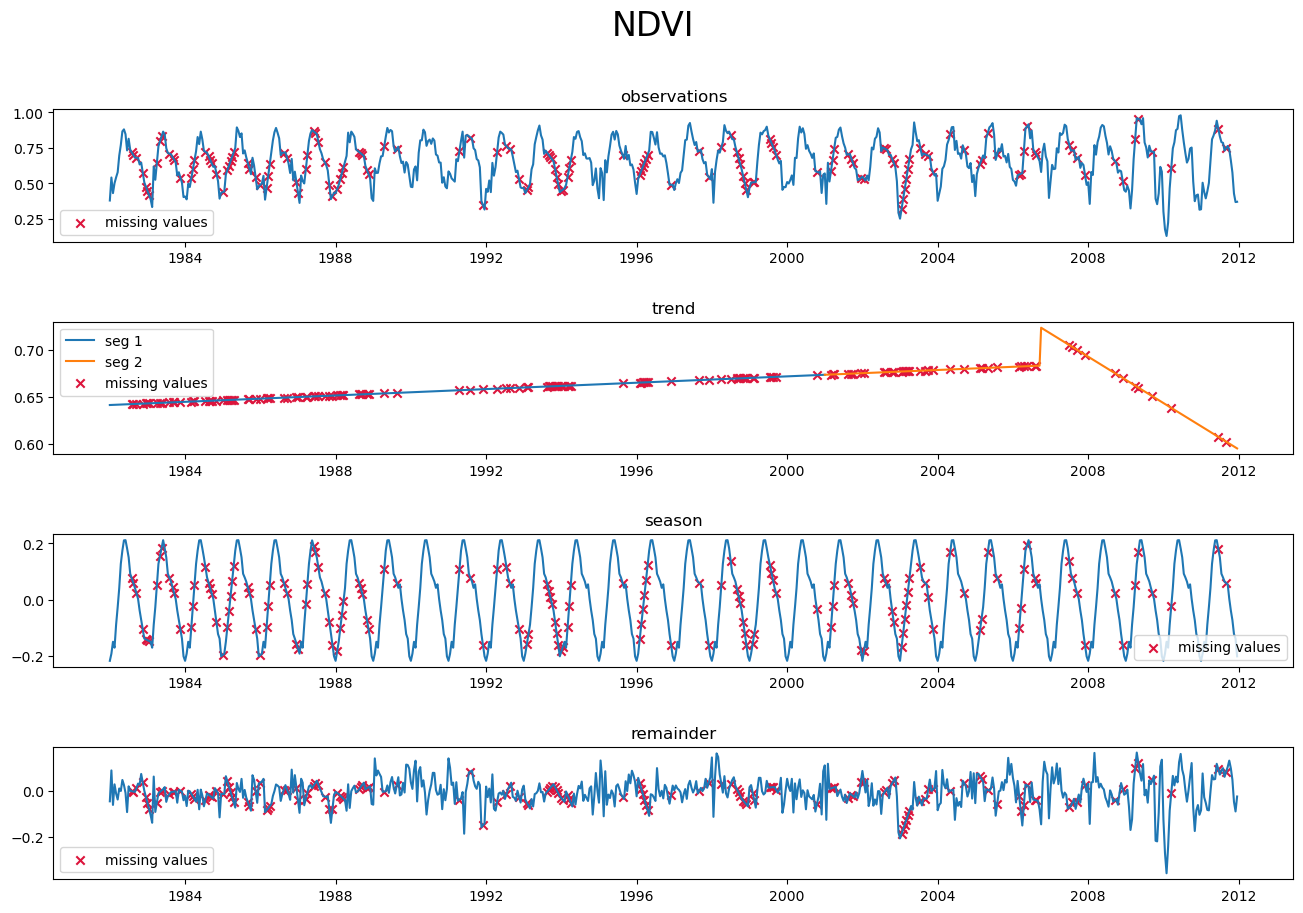
\includegraphics[width=0.9\textwidth]{imgs/ndvi.png}
  \caption{A random NDVI time series with missing values. Frequency is set to 24.
    There is a single breakpoint in the trend component. ``dummy'' seasonal model.}
\end{figure}
\end{frame}

\begin{frame}
  \frametitle{Trend Component}
  \begin{itemize}
  \item 
  We assume that $T_t$ is piecewise linear and has breakpoints $t_1^*,\hdots, t_m^*$,
  where $m$ is the number of breakpoints in the trend component and set $t_0^* = 0$.
  Then, the trend component can be described as
  \[
  T_t = \alpha_j + \beta_j t \quad \text{for}\quad t^*_{j-1}<t\leq t_j^*
  \]
  where:
  \begin{itemize}
  \item $j$ is the number of the next breakpoint, i.e. $j = 1,...,m$.
  \item $\alpha_j$ and $\beta_j$ are the corresponding linear coefficients
  \end{itemize}
  %% \item In matrix form:
  %%   \[
  %%   \mathrm{T} = \mathrm{X} \beta
  %%   \]
  %%   \[
  %%   \mathrm{T} = 
  %%   \begin{bmatrix}
  %%     T_1 \\
  %%     T_2 \\
  %%     \vdots \\
  %%     T_n 
  %%   \end{bmatrix}
  %%   \quad
  %%   \mathrm{X} = 
  %%   \begin{bmatrix}
  %%     1 & T_1 \\
  %%     1 & T_2 \\
  %%     \vdots & \vdots \\
  %%     1 & T_n 
  %%   \end{bmatrix}
  %%   \quad
  %%   \beta =
  %%   \begin{bmatrix}
  %%     \alpha \\
  %%     \beta 
  %%   \end{bmatrix}
  %%   \]
  %% \item 
  %%   One way, in which we can characterize the abrupt changes in the trend component is by
  %%   calculating the magnitude of the change:
  %%   \[
  %%   \operatorname{Magnitude}(j) = T_{j-1} - T_{j} = (\alpha_{j-1} - \alpha_j) + (\beta_{j-1} - \beta_j)t
  %%   \]
  %%   where $j = 1,...,m$.
  \end{itemize}
\end{frame}

\begin{frame}
  \frametitle{Seasonal Component}
  \begin{itemize}
  \item 
    There are two seasonal models that were introduced by Verbesselt et al.:
    Harmonic and ``dummy''. This presentation only covers the former.
    \item 
      The breakpoints in the seasonal component can occur at different times than the
      breaks in the trend component. Let
      $t_1^{\#},\hdots, t_p^{\#}$ be the breakpoints in the seasonal component,
      where $p$ is the number of breakpoints and $t_0^{\#} = 0$.
    \item 
      
      For $t_{j-1}^{\#} < t \leq t_j^{\#}$, the seasonal term can be expressed as:
    \[
    S_t =
    \sum_{k=1}^{K}\left[\gamma_{j, k} \sin \left(\frac{2 \pi k t}{s}\right)+
      \theta_{j, k} \cos \left(\frac{2 \pi k t}{s}\right)\right]
    \]
where
\begin{itemize}
\item $K$ is the harmonic term, i.e. the number of pairs of harmonic terms:
  ($K=3$ is used in BFAST)
\item $\gamma_{j, k}$ and $\theta_{j, k}$ are the seasonal coefficients
\item $t$ is the observation time.
\item $s$ is the period of seasonality (e.g. number of observations per year)
\end{itemize}
  \end{itemize}
\end{frame}

%% \begin{frame}
%%   \frametitle{Seasonal Component - Harmonic Model Continued}
%%   In order to apply the model to the time-series s.t. it could be used by the
%%   breakpoint estimation algorithm, we need to compute the matrix form of the
%%   harmonic model (for $K=3$):
%%   \[
%%   X_{h} =
%%   \begin{bmatrix}
%%     \sin\nicefrac{2 \pi}{f} & \cos\nicefrac{2 \pi}{f} & \sin\nicefrac{4 \pi}{f} & \cos\nicefrac{4
%%       \pi}{f} &  \sin\nicefrac{6 \pi}{f} & \cos\nicefrac{6 \pi}{f} \\
%%     \sin\nicefrac{4 \pi}{f} & \cos\nicefrac{4 \pi}{f} & \sin\nicefrac{8 \pi}{f} & \cos\nicefrac{8
%%       \pi}{f} &  \sin\nicefrac{12 \pi}{f} & \cos\nicefrac{12 \pi}{f} \\
%%     \vdots & \vdots  & \vdots & \vdots & \vdots & \vdots \\
%%     \sin\nicefrac{2 \pi n}{f} & \cos\nicefrac{2 \pi n}{f} & \sin\nicefrac{4 \pi n}{f} &
%%     \cos\nicefrac{4 \pi n}{f} &  \sin\nicefrac{6 \pi n}{f} & \cos\nicefrac{6 \pi n}{f}
%%   \end{bmatrix}
%%   \]
%%   $X_h$ has $n$ rows and $2K$ columns.
%% \[
%% \hat{S} = X_{\text{h}} \omega
%% \]
%% where $\omega$ is a $(1 \times 2K)$ vector
%% $(\gamma_{1, 1}, \; \theta_{1, 1},\;  \gamma_{1, 2},\;  \theta_{1, 2},\; \gamma_{p, 3},\;  \theta_{p, 3})^{\top}$
%% \end{frame}

\begin{frame}
  \frametitle{BFAST Algorithm Steps}
  \begin{itemize}
  \item \textbf{Estimate $S_t$ using STL decomposition, resulting in $\hat{S}_t$}
  \item Iterate, until the number and position of the breakpoints do
    not change during the iteration or the maximum allowed number of iterations
    is reached:
    \begin{enumerate}
    \item \textbf{Calculate the deasonalized time series: $V_t = Y_t - \hat{S}_t$}
    \item \textbf{Apply the OLS-MOSUM test} to $V_t$
      If the returned p-value is lower than the significance level $\alpha$,
      \textbf{estimate the number and position of the trend components} using the
      breakpoint estimation algorithm by Bai and Perron.
    \item \textbf{Compute the trend coefficients} $\alpha_j$ and $\beta_j$ for
      $j = 1, \hdots, m$ using linear regression. Set the trend estimate
      $\hat{T}_t = \hat{\alpha}_j + \hat{\beta}_j t$ for
      $t = t^*_{j-1} + 1, \hdots, t^*_j$.
    \item \textbf{Calculate the detrended time series}: $W_t = Y_t - \hat{T}_t$
    \item \textbf{Apply the OLS-MOSUM test} to $W_t$
    If the test results show that the breakpoints are present in the
      seasonal data, \textbf{estimate the number and position of the
      breakpoints in the seasonal component} using the breakpoint estimation
      algorithm
    \item \textbf{Compute the coefficients for the seasonal component
      and reconstruct $\hat{S}_t$} from the chosen seasonal model and seasonal
      coefficient
  \end{enumerate}
%% \item \textbf{Return} $\hat{T}_t$, $\hat{S}_t$, $(t_1^*, \hdots, t_m^*)$, $(t_1^{\#}, \hdots, t_p^{\#})$
  %% and the maximum breakpoint magnitude.
\end{itemize}

\end{frame}

\end{document}


%% \documentclass[main.tex]{subfiles}

\begin{document}
\chapter{Implementation}
\label{chap:implementation}
Both BFAST0n and BFAST algorithms were implemented in Python 3.8.3 using
\texttt{numpy}, \texttt{statsmodels}\cite{statsmodels} for all the computation
and \texttt{matplotlib} for all the plotting. The implementation is based on the
original R implementation of BFAST and BFAST0n by Verbesselt et al.
\cite{bfast-github} and the \texttt{strucchange} library by Zeileis
\cite{strucchange_code}.

\biblio
\end{document}


%% \documentclass[main.tex]{subfiles}

\begin{document}
\chapter{Validation}
\label{chap:validation}
In order to validate the implementation of BFAST and BFAST0n, four datasets were
chosen. Each of the datasets was chosen to test a specific
property of the algorithm. Three of the datasets were
taken from the paper by Verbesselt et al. \cite{bfast} and one from the standard
dataset library for the R programming language \cite{r-datasets}. The results were compared to
the same data applied to the original R-implementation of BFAST and BFAST0n
\cite{bfast-github}. Both mine and R implementation find exactly same
breakpoints for the same input and parameter values. There are however some
small differences in the decomposition due to different implementations of STL
and linear regression. Chapter \ref{chap:implementation} elaborates on both of
these points. This chapter only covers the validation of the BFAST algorithm,
but the BFAST0n implementation was tested in a similar manner.

\section{\texttt{nile}}
\label{sec:val_nile}
Measurements of the annual flow of the river Nile at Aswan (formerly Assuan),
1871–1970. With apparent changepoint near 1898. From \cite{r-datasets}. There is
no seasonal component, since there is only a single observation each year. This
tests the breakpoint estimating capacity without STL and seasonal model.
Following parameter values were used:
\begin{itemize}
\item \texttt{season}= "none"
\item $\alpha = 0.05$
\item $h = 0.15$
\end{itemize}
The results can be seen on Figure \ref{plt:nile}.
\begin{figure}
  \centering
  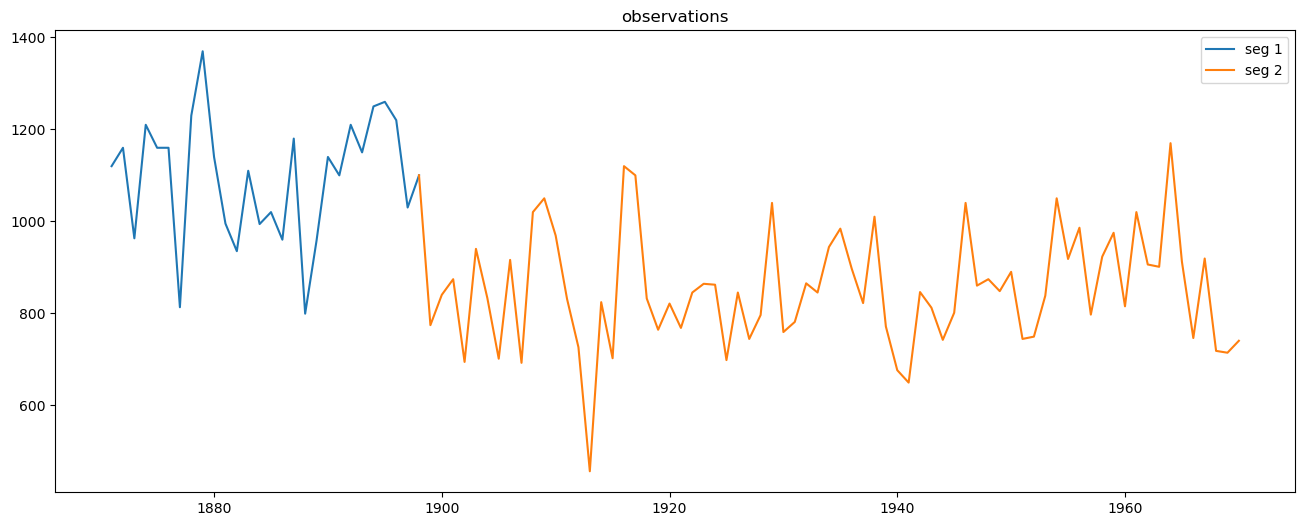
\includegraphics[width=\textwidth]{imgs/nile.png}
  \caption{Result of applying BFAST to the \texttt{nile} dataset.
    \texttt{season} = ``none'' had been chosen, hence no decomposition was done}
  \label{plt:nile}
\end{figure}

\section{\texttt{harvest}}
\label{sec:val_harvest}
16-day NDVI Time Series for a Pinus Radiata Plantation, with approximately 23
observation per year from \cite{bfast}. There are 4 breakpoints in the trend
component exclusively. The results can be seen on Figure \ref{plt:harvest}
Following parameter values were used:
\begin{itemize}
\item \texttt{season}= ``harmonic''
\item $\alpha = 0.05$
\item $h = 0.15$
\end{itemize}

\begin{figure}
  \centering
  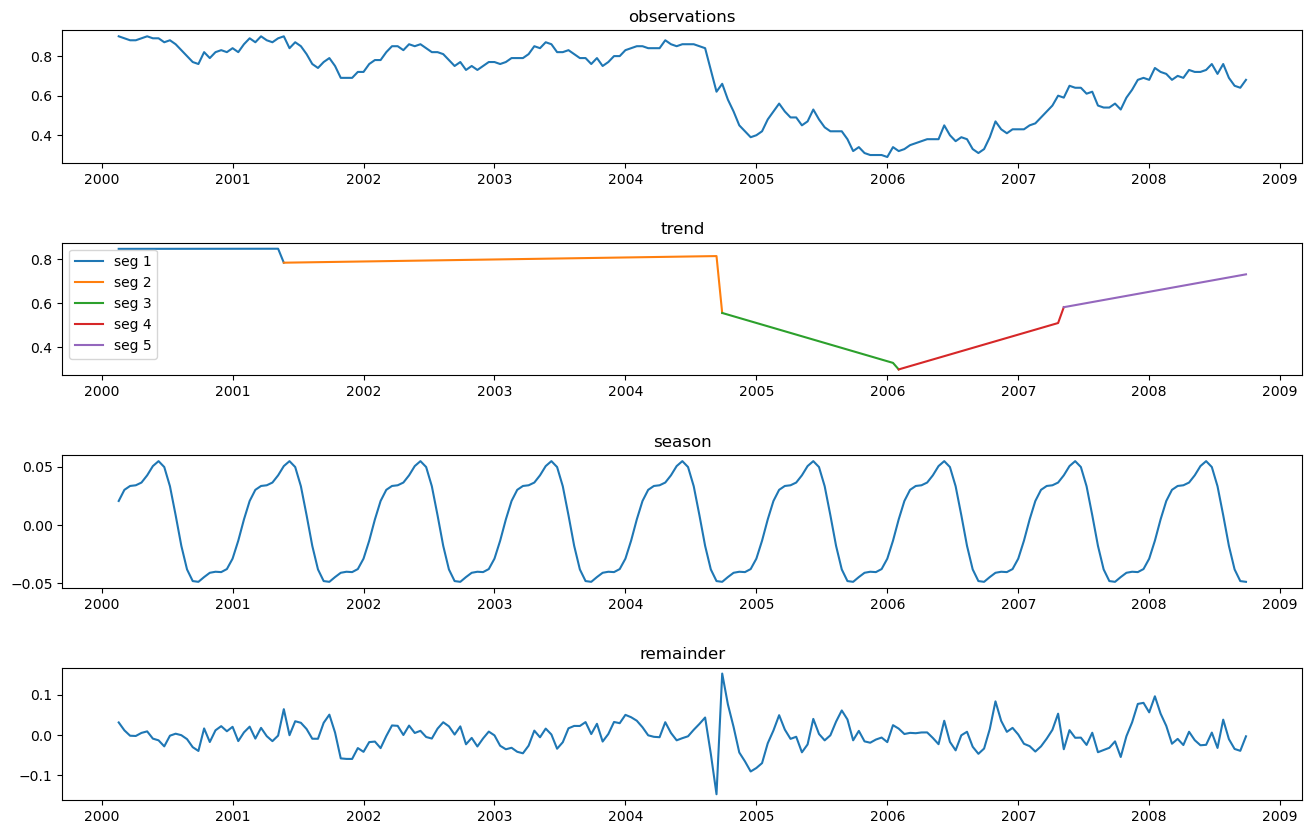
\includegraphics[width=\textwidth]{imgs/harvest.png}
  \caption{Result of applying BFAST to the \texttt{harvest} dataset}
  \label{plt:harvest}
\end{figure}

\section{\texttt{simts}}
\label{sec:val_simts}
Simulated seasonal 16-day NDVI time series from \cite{bfast}. The seasonal
component has a single breakpoint that is difficult to detect. Hence, following
parameter values were used:
\begin{itemize}
\item \texttt{season}= "harmonic"
\item $\alpha = 0.35$
\item $h = 0.3$
\item \texttt{max\_iter} = 2
\end{itemize}
The results can be seen on Figure \ref{plt:simts}.

\begin{figure}
  \centering
  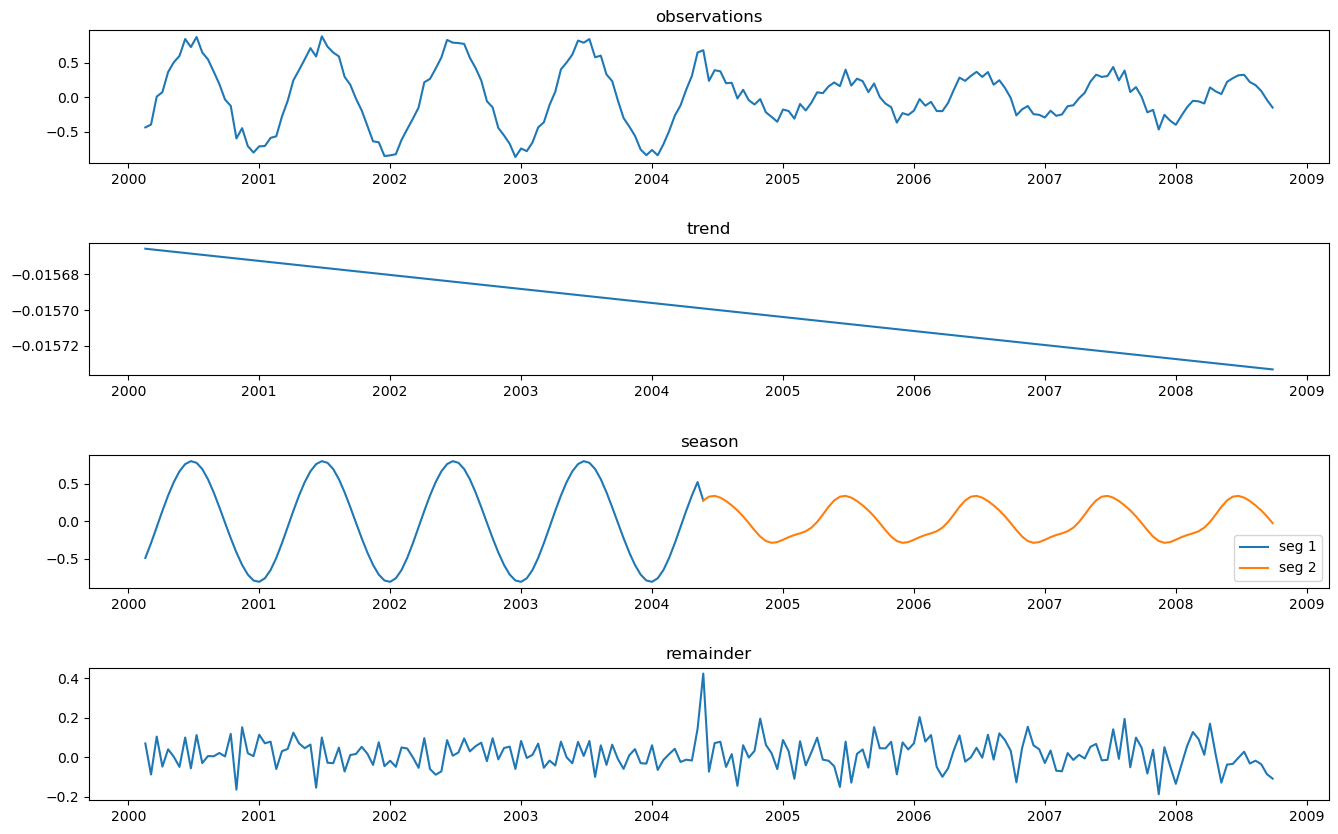
\includegraphics[width=\textwidth]{imgs/simts.png}
  \caption{Result of applying BFAST to the \texttt{simts} dataset}
  \label{plt:simts}
\end{figure}

\section{\texttt{ndvi}}
\label{sec:val_ndvi}
A random NDVI time series with missing values. BFAST should pass the missing
values into the seasonal, trend and remainder components, and my implementation
accomplishes that. Frequency is set to 24.
There is a single breakpoint in the trend component.
Source: \cite{bfast}. Following parameter values were used:
\begin{itemize}
\item \texttt{season}= ``dummy''
\item $\alpha = 0.05$
\item $h = 0.15$
\end{itemize}
The results can be seen on Figure \ref{plt:ndvi}.
\begin{figure}
  \centering
  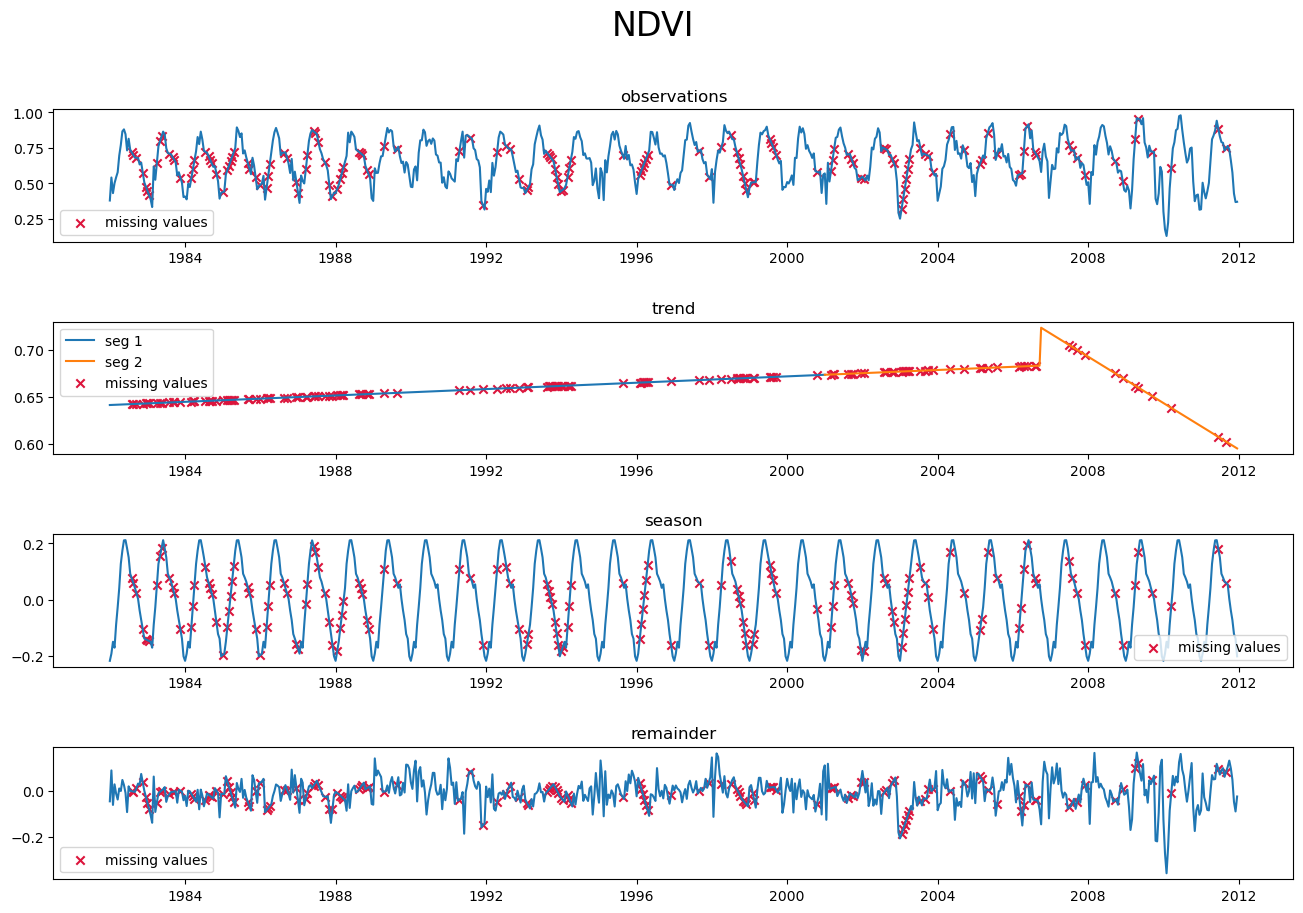
\includegraphics[width=\textwidth]{imgs/ndvi.png}
  \caption{Result of applying BFAST to the \texttt{NDVI} dataset. Red crosses
    denote the missing values}
  \label{plt:ndvi}
\end{figure}


\biblio
\end{document}


%% \documentclass[main.tex]{subfiles}

\begin{document}
\chapter{Conclusion and Future Work}
\label{chap:conclusion_and_future_work}
I have completed a working prototype implementation of BFAST and BFAST0n
structural change detection algorithms by Verbesselt et al. \cite{bfast} in
Python. My implementation was validated using the datasets from the original
paper and results were compared to the original R implementation \cite{bfast-github}.

This report chronicles my implementation of the BFAST and BFAST0n and covers the
underlying theory of both algorithms. In particular, I describe in detail the
concrete steps of each component of BFAST. This includes the STL decomposition
algorithm \cite{stl}, OLS-MOSUM test by Achim Zeileis \cite{strucchange}, the
breakpoint estimation algorithm by Bai and Perron \cite{bai_perron} and BFAST
itself. The description of the concrete algorithm steps can be helpful to a
potential programmer that would like to implement one of the algorithms
without diving too deep into the statistical theory. 

However, some parts of the algorithm have been omitted and should be added in
the future. This includes the computation of the confidence intervals for the
breakpoints in the algorithm by Bai and Perron. The underlying theory was too
overwhelming for a person without a background in either statistics or
econometrics and therefore was given the lowest priority, since both BFAST and
BFAST0n can function without it.

Moreover, the differences between the BFAST and BFAST Monitor \cite{bfast_monitor}
approach are not covered in this report either, since it would be a crucial part of my
MSc thesis, and this project is focused around the theory of the BFAST and its components.

Since performance was not the aim of this particular project, this
implementation is rather slow and is comparable to the original R
implementation. It struggles with any time series with more than 500
observation (as demonstrated by the \texttt{NDVI} dataset. In addition, the Python
implementation is about 30\% slower than the original implementation, since
the original uses C++ for some of its most resource-demanding procedures.

The outcome of this project forms a solid foundation for
the future work, where a parallelized, GPU-based implementation would be
developed and compared to the existing massively-parallel implementation of BFAST-Monitor.

\biblio
\end{document}


\bibliography{mybib}{}
\bibliographystyle{plain}
\newpage
\appendix
\documentclass[main.tex]{subfiles}

\begin{document}
\chapter{How to Run the Tests}
\label{a_chap:source_code_overview}
Tests for each file in the \emph{src} directory are contained withing that
source file. In order to run the test, run:
\begin{verbatim}
python file.py
\end{verbatim}
In order to get the more verbose output, run:
\begin{verbatim}
python file.py --log=INFO
\end{verbatim}
In order to see the debug information, run:
\begin{verbatim}
python file.py --log=DEBUG
\end{verbatim}

\biblio
\end{document}


\end{document}


% }

%% \begin{figure}
%%   \centering
%%   \begin{subfigure}[b]{\textwidth}
%%     \centering
%%     \includegraphics[scale=0.8]{handin/plt51}
%%     \caption{Classification of the training set}
%%   \end{subfigure}
%%   \begin{subfigure}[b]{\textwidth}
%%     \centering
%%     \includegraphics[scale=0.8]{handin/plt52}
%%     \caption{Classification of the test set}
%%   \end{subfigure}
%%   \caption{Exercise 5: Logistic Regression Applied to the Datasets}
%%   \label{plt5}
%% \end{figure}

%% \begin{lstlisting}[caption="Calculation of g"]
%% def calc_g(Xs, y, w):
%%     N = np.shape(Xs)[0]
%%     # use matrix X of xs instead of for-loop = much faster
%%     X = np.c_[Xs, np.ones(N)]
%%     num = y.T * X
%%     denum = 1 + np.exp(y * (w @ X.T))
%%     M = num.T/denum
%%     # return mean of each row
%%     return (-1 * np.mean(M, axis=1))
%% \end{lstlisting}
